\subsection{Overlap}
\label{sec:accuracy}
%We run our algorithm on the Google dataset
%%using either MI or TF-IDF as the confidence function
%to obtain action concepts for $k\in\{5, 10, 15, 20\}$,
%and for both subjects and objects as well as for triplets.
%We show the degree of overlaps for each verb
%of all verbs in
%Verb-20.
%\KZ{We should report the total, average number of concepts and
%their standard deviation in
%our lexicon. This is to show that the scale of our lexicon is much
%larger than FrameNet. FrameNet has 1200 Frames and 13,000 senses.}
%We set the parameter $\tau=0.2$, which will be discussed
%in \ref{sec:decision_tau}.
%As an example, \tabref{tab:top5result} shows the
%top 5 object concepts for Verb-20 extracted using MI on Web data.
%In this section, we show the accuracy of the action concepts
%and the degree of their overlaps for each verb by human judgment,
%as well as how to tune the parameters $\tau$ and $k$ for constructing
%the complete lexicons.

%This score measures the difference between the prior probability
%$p(c)$ and posterior distribution
%$p(c|p)$. A large difference stands for high co-occurrence of $c$ and $v$,
%and hence the class and the verb are strongly coupled.

%Since we mainly focus on evaluating the object concepts extracted by
%our approaches, we abuse using the term \emph{argument}
%to refer to object of the verbs in the following experiments.
%\begin{table}[th]
%\caption{Top 5 Object Concepts Extracted by AC on the Web Data}
%\center
%\small
%% Table generated by Excel2LaTeX from sheet 'Sheet1'
%\begin{tabular}{|l|l|}
%    \hline
%    Verb  & Object Concepts\\
%    \hline \hline
%    bring	&person,issue,item,material,factor\\
%    \hline
%    carry	&weapon,product,name,species,factor\\
%    \hline
%    connect	&device,system,component,area,technology\\
%    \hline
%    cut	&material,part,factor,accessory,issue\\
%    \hline
%    define	&group,event,feature,factor,document\\
%    \hline
%    eat	&food,plant,dish,ingredient,flavor\\
%    \hline
%    help    &person,community,company,organization,group\\
%    \hline
%    hit	&place,feature,artist,application,item\\
%    \hline
%    keep	&information,name,item,area,feature\\
%    \hline
%    operate	&system,facility,service,device,technology\\
%    \hline
%    perform	&task,procedure,service,activity,method\\
%    \hline
%    play    &game,character,player,activity,name\\
%    \hline
%    read	&book,information,newspaper,site,classic\\
%    \hline
%    release	&information,name,product,material,player\\
%    \hline
%    report	&crime,event,infection,species,organization\\
%    \hline
%    select	&item,name,topic,feature,company\\
%    \hline
%    spend	&time,money,fund,occasion,festival\\
%    \hline
%    submit	&information,document,datum,documentation,material\\
%    \hline
%    visit	&site,place,community,attraction,name\\
%    \hline
%    wear	&clothing,item,style,accessory,device\\
%    \hline
%    \end{tabular}%
%\label{tab:top5result}
%\end{table}

%
%\subsubsection{Accuracy}
%We use precision, recall and $F_1$ measure to evaluate our
%algorithm and the generated lexicon.
%
%\textbf{Precision}:
%%We use precision to evaluate the quality of concepts produced by each
%%algorithm.
%For a given verb, a good concept for an argument type
%(either subject or object) not only covers as many as arguments in the dataset,
%but also contains few entities that are invalid for that verb.
%The precision score for each verb is:
%\[
%Precision = \frac{\sum_{c \in C_k}|E_c|\times Precision(c)}
%{\sum_{c \in C_k}{|E_c|}},
%\]
%\[
%Precision(c)=\frac{|\mbox{Entities in~} c
%\mbox{~which are correct arguments}|}{|E_c|}.
%\]
%%where $|E_c|$ is the number of entities in concept $c$ and
%%$C_k$ is the set of 10 argument concepts discovered by the algorithms.
%%We build a ground truth dataset for Verb-20 by
%Annotating all entities for each concept needs a large
%amount of human efforts. We use a sample strategy to
%estimate $Precision(c)$ for a concept $c$. Specifically,
%we sample 10 entities from each of the $k$ argument concepts
%for each verb learned by the AC and SP.
%%discovered by the algorithm.
%%To make more typical entities to be more easily sampled out,
%%the sampling is conducted according to the typicality of the entities.
%%The resulting annotation set comprises 2000 unique entities.
%Each entity is then labeled whether it is a correct argument to the
%verb by majority of three human judges.
%We compare the our algorithm, i.e., AC(MI) and AC(TF-IDF) to
%SP in terms of precision.
%The overall precision of the 20 verbs
%is reported in \figref{fig:precision_ngram}.
%%For all the algorithms, we keep the top-k concepts for the argument of
%%each verb.
%%For the Web data, as the number of concepts $k$ grows, the precision generally
%%decreases in all methods. For the Google data,
%The precision is relatively
%stable across different values of $k$.
%%This phenomenon indicates that the smaller scale of
%%the data causes smaller disparity of the overall quality for different size of concepts we get.
%AC(MI) outperforms AC(TF-IDF) and
%SP by significant margins. AC(TF-IDF) gives low precision,
%perhaps because the TF-IDF scoring doesn't penalize the incorrect arguments
%sufficiently but instead prefers to select more general
%concepts to maximize the score (\eqnref{eq:approxf}).
%%The greedy solution loses in terms of precision
%%comparing to local search and selectional preference because it prefers
%%to select general concepts to minimize the number of concepts.
%%Simulated annealing is able to jump out of the local optimal and
%%find a solution that close to the global optimal.
%%The comparison among the three approaches on web sentence dataset
%%shows that our local search algorithm is enable to find concepts
%%with proper granularity, i.e., covering most correct arguments but
%%less incorrect arguments. We also compare the precision of
%%applying local search to web sentence data with that to Google
%%syntactic N-grams.
%
%\textbf{Recall}: Recall measures the coverage of
%correct arguments of a verb by the lexicons.
%We create two gold standard datasets to evaluate
%the recall of action concepts.
%We manually label 100 correct arguments for each
%verb in Verb-20.
%These correct arguments are collected randomly and evaluated
%by three human judges. With the ground truth, we check
%if those correct arguments are covered by one of the concepts
%extracted by each algorithm.
%The definition of recall for each verb
%is computed as below.
%$$
%Recall=\frac{\sum_{a \in A_v}{I(a,C)}}{|A_v|},
%$$
%%where
%%$A$ is the set of arguments in the web/Google dataset for the verb;
%%function $I(a,C)$ is defined as:
%$$
%I(a,C)=
%\begin{cases}
%1 & \mbox{if}~ \exists c \in C\ \mbox{and}\ a\ \mbox{IsA}\ c,\\
%0 & \mbox{otherwise.}
%\end{cases}
%$$
%
%We report the recall of our algorithms %, i.e., AC(MI) and AC(TF-IDF)
%as well as SP in \figref{fig:recall_ngram}.
%%Greedy solution achieves a very high recall, because
%%it prefers larger concepts. Local search and selectional
%%preference performs similar in terms of recall.
%On both datasets, AC(MI) and AC(TF-IDF) perform much better than SP.
%Using TF-IDF as the confidence function achieves a higher recall, because it
%tends to select larger concepts, which may decrease the precision
%on the contrary as we have discussed.
%
%\textbf{$F_1$ measure}: We examine the $F_1$ measure to
%incorporate the precision and recall for an overall
%evaluation of the accuracy of the algorithms.
%%$F_1$ is
%%define as follows:
%%$$
%%F_1=\frac{2\cdot Precision \cdot Recall}{Precision + Recall}.
%%$$
%The $F_1$ measure of all three algorithms are summarized in
%\figref{fig:f1_ngram}.
%%Greedy solution is fast and achieves good accuracy
%%in the top three concepts, while appears to be less efficient
%%when the number of concepts become large.
%%Local search outperforms
%%selectional preference in all settings.
%From the figures, we conclude that AC(MI) and AC(TF-IDF) achieve
%higher accuracy than SP.
%%and AC(MI) performs better than AC(TF-IDF).
%Because MI has better capability of suppressing low quality entities
%than TF-IDF, it achieves the highest overall accuracy.
%Generally, AC achieves much higher and more stable accuracy
%with different values of $k$ than SP.
%This is because we consider the concept diversity of the generated concept
%lexicon, while SP just selects the top concepts with the highest
%preference scores. As such, SP concepts tend to have higher overlap
%with each other as we show next.
%%\begin{figure*}[th]
%%\begin{minipage}[t]{0.5\columnwidth}
%%\centering
%%\epsfig{file=figure/precision_web.eps,width=\columnwidth}
%%\caption{Precision - Web}
%%\label{fig:precision_web}
%%\end{minipage}
%%\begin{minipage}[t]{0.5\columnwidth}
%%\centering
%%\epsfig{file=figure/recall_web.eps,width=\columnwidth}
%%\caption{Recall - Web}
%%\label{fig:recall_web}
%%\end{minipage}
%%\begin{minipage}[t]{0.5\columnwidth}
%%\centering
%%\epsfig{file=figure/f_web.eps,width=\columnwidth}
%%\caption{$F_1$ Measure - Web}
%%\label{fig:f1_web}
%%\end{minipage}
%%\begin{minipage}[t]{0.5\columnwidth}
%%\centering
%%\epsfig{file=figure/overlap_web.eps,width=\columnwidth}
%%\caption{Overlap - Web}
%%\label{fig:overlap_web}
%%\end{minipage}
%%\end{figure*}
%

The overlap score reflects the concepts diversity of the generated lexicon.
The intuition is that the more overlap the pairwise concepts have,
the lower diversity does the lexicon have.
In this section, we evaluate the average pairwise overlap between
extracted action concepts.
%Ideally the intersection between every two concepts in the result
%should be as small as possible, which means each concept should
%correspond to a distinct meaning.
%We compute the average overlap score as:
%\[
%Overlap_{avg} = \frac{2\times \sum_{c_1,c_2\in C_k}{Overlap(c_1,c_2)}}{k(k-1)},
%\]
%where $C_k$ is the set of top $k$ argument concepts discovered by
%the algorithms; $Overlap(c_1,c_2)$ is computed by \eqnref{eq:overlap}.

We use class-based selectional preference (SP) proposed by
Resnik et al.\shortcite{resnik1996selectional}
as the baseline method for conceptualizing verb arguments in the rest of
the evaluation section because it can
produce human readable classes/concepts.
Notice that most of recent techniques for SP are not class-based,
and thus cannot generate human readable classes for lexicon
construction.
%Class-based SP computes the selectional association between a
%semantic class $c$ and a predicate $p$ as:
%\begin{equation}
%A(p,c)=\frac{Pr(c|p)\log\frac{Pr(c|p)}{Pr(c)}}
%{\sum_{c'\in C}{Pr(c'|p)\log\frac{Pr(c'|p)}{Pr(c')}}},
%\end{equation}
%where $C$ is the collection of semantic classes.

The overlap scores of our algorithm and SP are shown in \figref{fig:overlap_ngram}.

\begin{figure}[th]
\centering
\epsfig{file=figure/overlap_new.eps,width=0.7\columnwidth}
\caption{Overlap}
\label{fig:overlap_ngram}
\end{figure}

%The intuition is that, if there is no overlap between
%every two concepts, each argument will be covered by only one concept,
%then overlap score will be 0 which is the best.
%The more overlap, the more concepts one object being covered,
%so that the overlap score will be high. The overlap score of action concepts extracted by the three algorithms
%as reported in \figref{fig:overlap_web}.
%\KZ{Need to revise the following:
%Most of the verbs do not overlap in greedy solution,
%because when we pick a concept we choose from concepts that do not violate the overlap
%constrain. Overlap of local search is slightly higher than GS, but it still guarantees
%the overlap constrain. In contrast, selectional preference tends to generate general
%concepts which results in a high overlap score.
%}
\KQ{Rewrite the following according to the results}
The concepts generated by AC(MI) overlap much less with each other than
AC(TF-IDF) or SP. Because SP does not consider the diversity of concepts,
the Overlap score is much higher. The SP lexicon thus contains many concepts
possessing the same or very similar meanings.
As AC(TF-IDF) prefers general concepts, the Overlap score is also
higher.

Since AC(MI) generally outperforms AC(TF-IDF) in both accuracy and
overlap, MI is adopted as the confidence function in all subsequent experiments.

%As $k=10$ generally produces good $F_1$ score and reasonable overlaps, in the
%following experiments, unless otherwise noted, $k=10$.

%\subsubsection{Tuning Parameters}
%Two parameters, namely $\tau$ and $k$, control the granularity of
%action concepts in the generated lexicon. We tune the two parameters
%on Verb-20 as follows. We obtain $\tau$ by fixing $k=10$ and computing
%$F_1$ score for the different settings of $\tau$ (from $0.05$ to $0.5$)
%on Verb-20 and observe that when $\tau=0.2$, the resulting
%lexicon has highest overall $F_1$. To decide $k$, we fix $\tau=0.2$ and
%tune gradient threshold discussed in \secref{sec:dpk}. Specifically, we
%find $k$ that achieves highest $F_1$ score for each verb, and
%compute the corresponding gradients according to \eqnref{eq:gradient}.
%We then choose the median value, i.e., 0.004, among these gradients
%as our threshold.

